\documentclass[conference]{IEEEtran}
% \IEEEoverridecommandlockouts

\usepackage{cite}
\usepackage{amsmath,amssymb,amsfonts}
\usepackage{algorithmic}
\usepackage{graphicx}
\usepackage{textcomp}
\usepackage{xcolor}
\usepackage{tabularx}
\usepackage{array}
\usepackage{subcaption}
\usepackage{booktabs}

\newcolumntype{Y}{>{\raggedright\arraybackslash}X}

\def\BibTeX{{\rm B\kern-.05em{\sc i\kern-.025em b}\kern-.08em
    T\kern-.1667em\lower.7ex\hbox{E}\kern-.125emX}}
\begin{document}

\begin{titlepage}
    \centering

    {\Huge\bfseries RES: A modular pipeline to recognise, encode and select relevant facts from clinical notes\par}
    \vspace{2cm}

    {\large
    A dissertation submitted in partial fulfilment of\par
    The requirement for the degree of\par
    MASTER OF SCIENCE in Artificial Intelligence\par
    in\par
    The Queen’s University of Belfast\par
    by\par
    Conor Brown\par
    4th September 2026
    }
\end{titlepage}


\title{RES: A modular pipeline to recognise, encode and select relevant facts from clinical notes\\}



\maketitle

\begin{abstract}
Clinical information extraction (IE) converts clinical 
narratives into structured facts. Large language models can 
do this with significantly less preprocessing than rules-based 
methods, but they introduce new classes of problems: 
hallucination, schema drift and overconfidence. We propose 
a hybrid system where the model recognises entities, interprets 
relations and provides evidence, and the rules normalise 
entities, verify evidence and apply policies to resolve conflicts. 
This modular system preserves the rich uncertainty captured 
in clinical narratives while producing auditable structured 
outputs that confirm to explicit rules. We use 2 public datasets 
of epilepsy letters to evaluate this system on two distinct tasks: 
(1) selecting the most important clinical fact among many and 
(2) building a broad inventory of clinical facts. We show that 
the combined system improved F1 by +0.05 vs. rules-only or 
LLM-only systems, while creating a rich evidence trail with an 
exact evidence score of >0.99. This transparent, 
evidence-grounded system is a step towards making more 
trustworthy systems for clinical use.
\end{abstract}

\begin{IEEEkeywords}
information extraction, neuro-symbolic, evidence verification, 
natural language processing
\end{IEEEkeywords}

\section{Introduction}

Clinical notes in electronic health records (EHRs) are 
among the most valuable sources of medical information 
available, recording diagnoses, medications, medical 
investigations and more in rich narrative form. This form is 
both a strength and a weakness. Patient demographics are 
routinely collected in structured forms for administrative 
purposes, and this structured form makes them easy to 
use in clinical research. Information about the patient's 
diagnoses and treatment outcomes often exist solely in 
narrative form in hospital discharge summaries or letters 
from clinicians. This makes them useful to deeply 
understand an individual patient, but very difficult to use 
to build a broad understanding of a patient population.

Epilepsy is one of the most common neurological 
diseases, affecting over [x]m people globally. Clinicians use 
the type of epilepsy, type of seizures and frequency of 
seizures to determine the severity of the patient's disease. [1]
Clinical trials typically use seizure freedom as their target 
outcome. [2] The only place this information is routinely 
recorded is in clinic letters from an epilepsy specialist to 
the patient's primary care doctor after the patient visits the 
clinic. To gather this information at scale, experts are 
required to complete manual chart review: review each 
letter, interpret the key details and translate them into a 
standard form. This process is costly, time-consuming, 
and error prone. [3] Making this information available in a 
structured form that you can query in a database to 
summarise, group and filter can make large-scale
research efforts viable.

To make this type of structured data available, there are
two broad approaches: collect the data in a structured 
form or process unstructured data into that form. It is 
simple to collect medication in a more structured form by 
using separate fields for medication, dose, unit and 
frequency, rather than writing 'Topiramate 100 mg BD' . 
Applying that to seizure frequency is more difficult 
because they are not simple facts to record in a single,
consistent form. A typical example is, \emph{"focal 
impaired-awareness seizures have been occurring 
more often, 2 times per week, whereas previously 
they only happened once or twice a month."} 
Imprecise language like this is known as hedging[5], 
and paradoxically, stripping it down to a single number 
would make it less precise and less useful. A system 
that enables clinicians to record these richer 
observations and then processes them into a 
standardised form is ideal.

Natural language processing (NLP) and the subdomain
of information extraction (IE) offers a solution for this. 
Rules-based methods have successfully extracted
information on medications and diagnoses, but struggled
with the imprecise language and diverse forms
of seizure frequency statements. '2 to 3 seizures a week', 
'frequent bouts of seizures' and '4 since her last visit' are
all valid descriptions of the same fact. Large language 
models (LLMs) have demonstrated significant 
improvements in semantic understanding than prior 
methods and have successfully extracted seizure 
frequency information, but they occasionally hallucinate
facts. Combining the semantic understanding of an LLM
with the transparency of a rules-based system could
provide the most accurate, trustworthy results.

Effective IE can be broken down into three key stages: 
recognising relevant candidate facts, encoding those facts 
into a particular form, and selecting which facts to keep 
and which to filter out. A clinic letter can contain multiple 
descriptions of seizures, some are historical events while 
others are current, some are certain seizures while others 
may be "absence-like episodes", some are describing the 
same event but in another context. Seizure frequencies 
can be expressed as a rate, a vague quantity and a 
duration. A transparent system would allow you to see not 
just the final answer, but which steps were taken to achieve 
it.

This paper evaluates the ideal combination of LLMs and 
rules across those three stages: recognition, encoding and 
selection. It was evaluated on two sets of annotated 
epilepsy clinic letters that reflect two common clinical IE 
tasks: producing a single label to determine a patient's 
current status, and producing a broad inventory of clinical 
facts, past and present. The paper demonstrates that a 
modular system combining LLMs and rules can extract 
information with comparable accuracy to past methods 
while preserving a richer evidence chain. The system 
is available as an open source package at INSERT LINK.
Figure 1 displays the web app illustrating some of that 
chain from evidence to final answer.

\section{Literature Review}

Epilepsy clinic letters contain facts about medication, 
diagnoses, investigations and seizure frequency, often
covering multiple time periods and with many hedged\cite{b1}
observations. Fonferko-Shadrach \emph{et al.} treat the 
letter as an inventory of supported facts across prescriptions, 
diagnosie, investigations and frequency\cite{b1,b2}. 
Xie \emph{et al.}~\cite{b3}, Holgate \emph{et al.}~\cite{b4}, and 
Gan \emph{et al.}~\cite{b3} treat it as one current 
seizure-frequency state. The decisions about which facts
to recognise, how to represent them and which facts to keep
in the final representation are often bundled into one 
single task definition. This paper demonstrates that 
breaking them up into discrete stages with explicit 
subjective choices can the make the system more 
transparent and flexible.

Wang \emph{et al.} define clinical IE as the automatic 
extraction and encoding of clinical information from 
text~\cite{b8}. Fu \emph{et al.} separate mention detection 
from concept encoding: the quoted span is distinct from
the coded concept~\cite{b6}. Xie \emph{et al.} extract a frequency 
sentence and then apply rules to encode it into a number~\cite{b9}. 
In much of the remaining epilepsy literature encoding is 
bundled into the extraction phase, with the model 
extracting e.g. '4 per month' from a raw statement 'about once 
a week'. When rules are used to format the answers, they are 
often described as simple post-processing steps for scoring 
instead of distinct stages in the pipeline. Those paper shows 
that separating recognition and encoding as separate stages 
preserves more of the evidence while still being able to 
encode it into the required form for downstream use.

DECIDE WHAT TO SAY ABOUT IAA

A number of methods have shown performance at 
or above human level. Fonferko-Shadrach \emph{et al.} 
reported the annotators found annotation difficult 
and seizure frequency was the most difficult. This was 
reflected in the inter annotator agreement (IAA) score
of 0.47 (moderate agreement) even after multiple phases 
of development of the guidelines to meet the annotators' 
needs.  Xie \emph{et al.} reported an overall pairwise F1
score of 0.44 on a task focused extracting seizure 
freedom, frequency and most recent seizure
statements and recommend double or triple annotation. 
This is a long-standing challenge in the field, as Grisham 
and Sundheim noted in 1996 ' it proved remarkably difficult
to formulate guidelines which were reasonably complete 
and consistent'. Despite levels of IAA of 0.5, the literature 
commonly reports that rules-based and LLM-based 
methods achieving F1 scores of 0.8 and above. 

INSERT A REVIEW OF EVALUATION PERFORMANCE

We have 8 different papers in the last 4 years with seizure frequency
performance results, but there is significant variance. 

Chiticariu \emph{et al.} show that academic papers tend to focus 
exclusively on benchmark accuracy, while practitioners tend 
to value transparency, configurability and efficiency at the 
cost of some accuracy. Fu \emph{et al.} show that this 
translates to the clinical setting too, and model interpretability 
is also a critical factor in successful deployment in clinical 
settings. Clinicians are highly trained in using deductive 
logic to draw conclusions and they expect systems to 
expose transparent, interpretable evidence that they can  
reliably use to make decisions that demand high 
accountability. Fonferko-Shadrach \emph{et al.} expose 
evidence spans as a consequence of using a rules-based 
system, and Gan \emph{et al.} utilise evidence spans as a 
training signal. This paper presents a transparent evidence 
chain from exact text to final answer as part of the core 
output to improve interpretability for downstream users.



Most papers present results of a system trained or tuned on 
one local corpus. Decker \emph{et al.} show that a highly 
tuned system on one set of epilepsy letters can perform 
significantly worse on a set from another epilepsy centre, 
with seizure-frequency $F_1$ dropping from 0.82 in-house 
to 0.40 at a second centre~\cite{b12}. This is further 
compounded by the fact that because medical data is highly
sensitive, most papers report results on private datasets 
that cannot be reproduced or evaluated on other systems. 
Fonferko-Shadrach \emph{et al.} and Gan \emph{et al.} 
are the two exceptions in this domain. This paper is the
first to assess a method on two distinct tasks using two
public datasets. 

\section{Methods}
\subsection{Data}

Two datasets were used in this paper. Both datasets
are collections of epilepsy clinic letters which record 
a UK patient's consultation with an epilepsy specialist, 
often a neurologist or specialist nurse. \cite{b2,b3} 
The NHS requires that clinic letters are sent to the 
patient's GP after all outpatient visits such as these. \cite{b13} 
They are often the only record of a patient's diagnoses,
treatments and outcomes in neurological disorders, 
and they are written in narrative form. Both datasets 
are synthetic letters modelled on real clinic letters, 
and they were annotated by trained researchers and 
clinicians. An example clinic letter is shown in Figure 1.

The primary difference in the two datasets is breadth
and depth of annotation. Fonferko-Shadrach \emph{et al.}
annotated a rich inventory of clinical facts, including the
current anti-seizure medications used, the types of epilepsy 
and seizures the patient was diagnosed with, the 
investigations used for diagnosis and the frequency of 
seizures. Multiple medications, diagnoses, investigations
and seizure frequency events can be recorded in a letter,
and each clinical fact has multiple attributes describing it. 
Figure 1 illustrates an example of multiple seizure frequency
events with multiple attributes linked to each. The task is 
to determine which clinical facts are relevant. This is referred 
to as the inventory dataset in this paper. Gan \emph{et al.} 
annotates a single label per letter with the patient's current
seizure frequency burden. The task is to determine which
fact to choose among many. If Gan \emph{et al.}'s annotation
was applied to the letter in Figure 1, the label would be '1 
per month'. This is referred to as the current frequency 
dataset.

The datasets also differ in how the letters were generated
and labelled. Fonferko-Shadrach \emph{et al.} produced
199 hand-authored letters by epilepsy specialists for the 
inventory dataset. Gan \emph{et al.} produced a much 
larger dataset of 15,099 letters using a combination of 10 
templates and 500 short descriptions of seizure frequency 
produced by GPT-5 for the current frequency dataset. A 
sample of 1,200 letters from Gan \emph{et al.} were used 
from current frequency, and all 199 letters from inventory. 
Table 1 summarises those details plus some statistics on
the length of the letters and the number of labels per letter.

\begin{table}[!t]
\caption{Dataset summary}
\label{tab:dataset}
\centering
\begin{tabularx}{\linewidth}{|Y|Y|Y|}
\hline
\textbf{} &
\textbf{Dataset 1} &
\textbf{Dataset 2} \\
\hline

Annotated clinical categories &
Medication, diagnosis, investigations and seizure frequency$^*$ &
Seizure frequency \\
\hline

Letter generation and annotation method  &
Human-written letters and labels &
AI-generated letters, human-written labels  \\
\hline

Number of letters (dev/test) &
199 (140/59) &
1,200 (750/450) \\
\hline

Median words per letter (range)  &
217 (49-693)&
400 (115-756) \\
\hline

Median number of annotated labels (range) &
6 (0-14)&
1 (1-1) \\
\hline
\end{tabularx}
{\raggedright\footnotesize $^*$The dataset includes 5 additional categories. This paper uses only these 4.}
\end{table}

\begin{figure*}[t]
    \centering

    
\includegraphics[width=\linewidth]{fig1.png}
    \caption{The left pane shows a clinic letter from Fonferko-Shadrach \emph{et al.} annotated for medications, diagnoses, 
    investigations and seizure frequencies. The right pane illustrates how multiple seizure events are represented in the schema.}
    \label{fig1}
\end{figure*}

Minimal preprocessing was applied to the raw data.
Dataset 1 stored the letters in raw .txt and annotations 
in .json files, while Dataset 2 stored both in a single 
.json file. Letters in both datasets are read in UTF-8 
format and minimally cleaned to correctly parse 
quotes, new lines, tabs, the $\leq$ sign and nulls. 
The raw letters were ingested in the pipeline in full; 
no tokenisation, section-splitting or truncation was
applied. 

Datasets were split up into stratified samples for 
separate development and test sets. Inventory 
was divided into 140 development/59 test sets. They 
were stratified by the existence of a seizure frequency 
mention, so c. 72\% of letters in both splits contain a 
seizure frequency fact. Current frequency was divided 
into 750 development letters and 450 test letters. They
were stratified by the kind of
seizure frequency fact so both sets consist of 
62\% with a frequency, 15\% seizure free, 13\% 
unknown and 10\% with no seizure frequency reference.
Seizure frequency was used to determine the
stratification because it is the most important 
clinical outcome for epilepsy patients and the 
only shared label between both datasets. 

\subsection{Architecture}

To trace the journey from raw evidence to final answer, 
the task was divided into three key stages: recognition,
encoding, selection. First, the pipeline identifies 
potential candidates that fit the description in the raw
text. Next, the pipeline takes the raw text from those
candidates and encodes them into the required form.
Finally, the pipeline determines which of those 
encoded facts meet the criteria for the final output. 
The specific configuration of the each stage is 
determined by the nature of the task: which labels to 
extract from the text, what schema to encode them 
into, and how many labels to output at the final stage.
The same modular architecture effectively describes
multi-label tasks such as inventory and single label 
tasks such as current frequency. Figure 2 illustrates the 
general architecture of the pipeline. 

There are two key benefits of breaking the task into 
three discrete stages: configurability and transparency. Past 
research has shown that entirely rules-based methods 
can successfully populate the inventory, while entirely
LLM-based methods can successfully extract the 
current frequency. While some methods have used a
combination of rules and LLMs to produce the final 
answer, none have empirically assessed the ideal 
combination of the two. This three-stage pipeline enables 
evaluation of the best combination overall, and specifically 
which component performs best at which stage. Table 2 
summarises the 3 main configurations of the pipeline 
evaluated in this paper. 

\begin{figure*}[t]
    \centering

    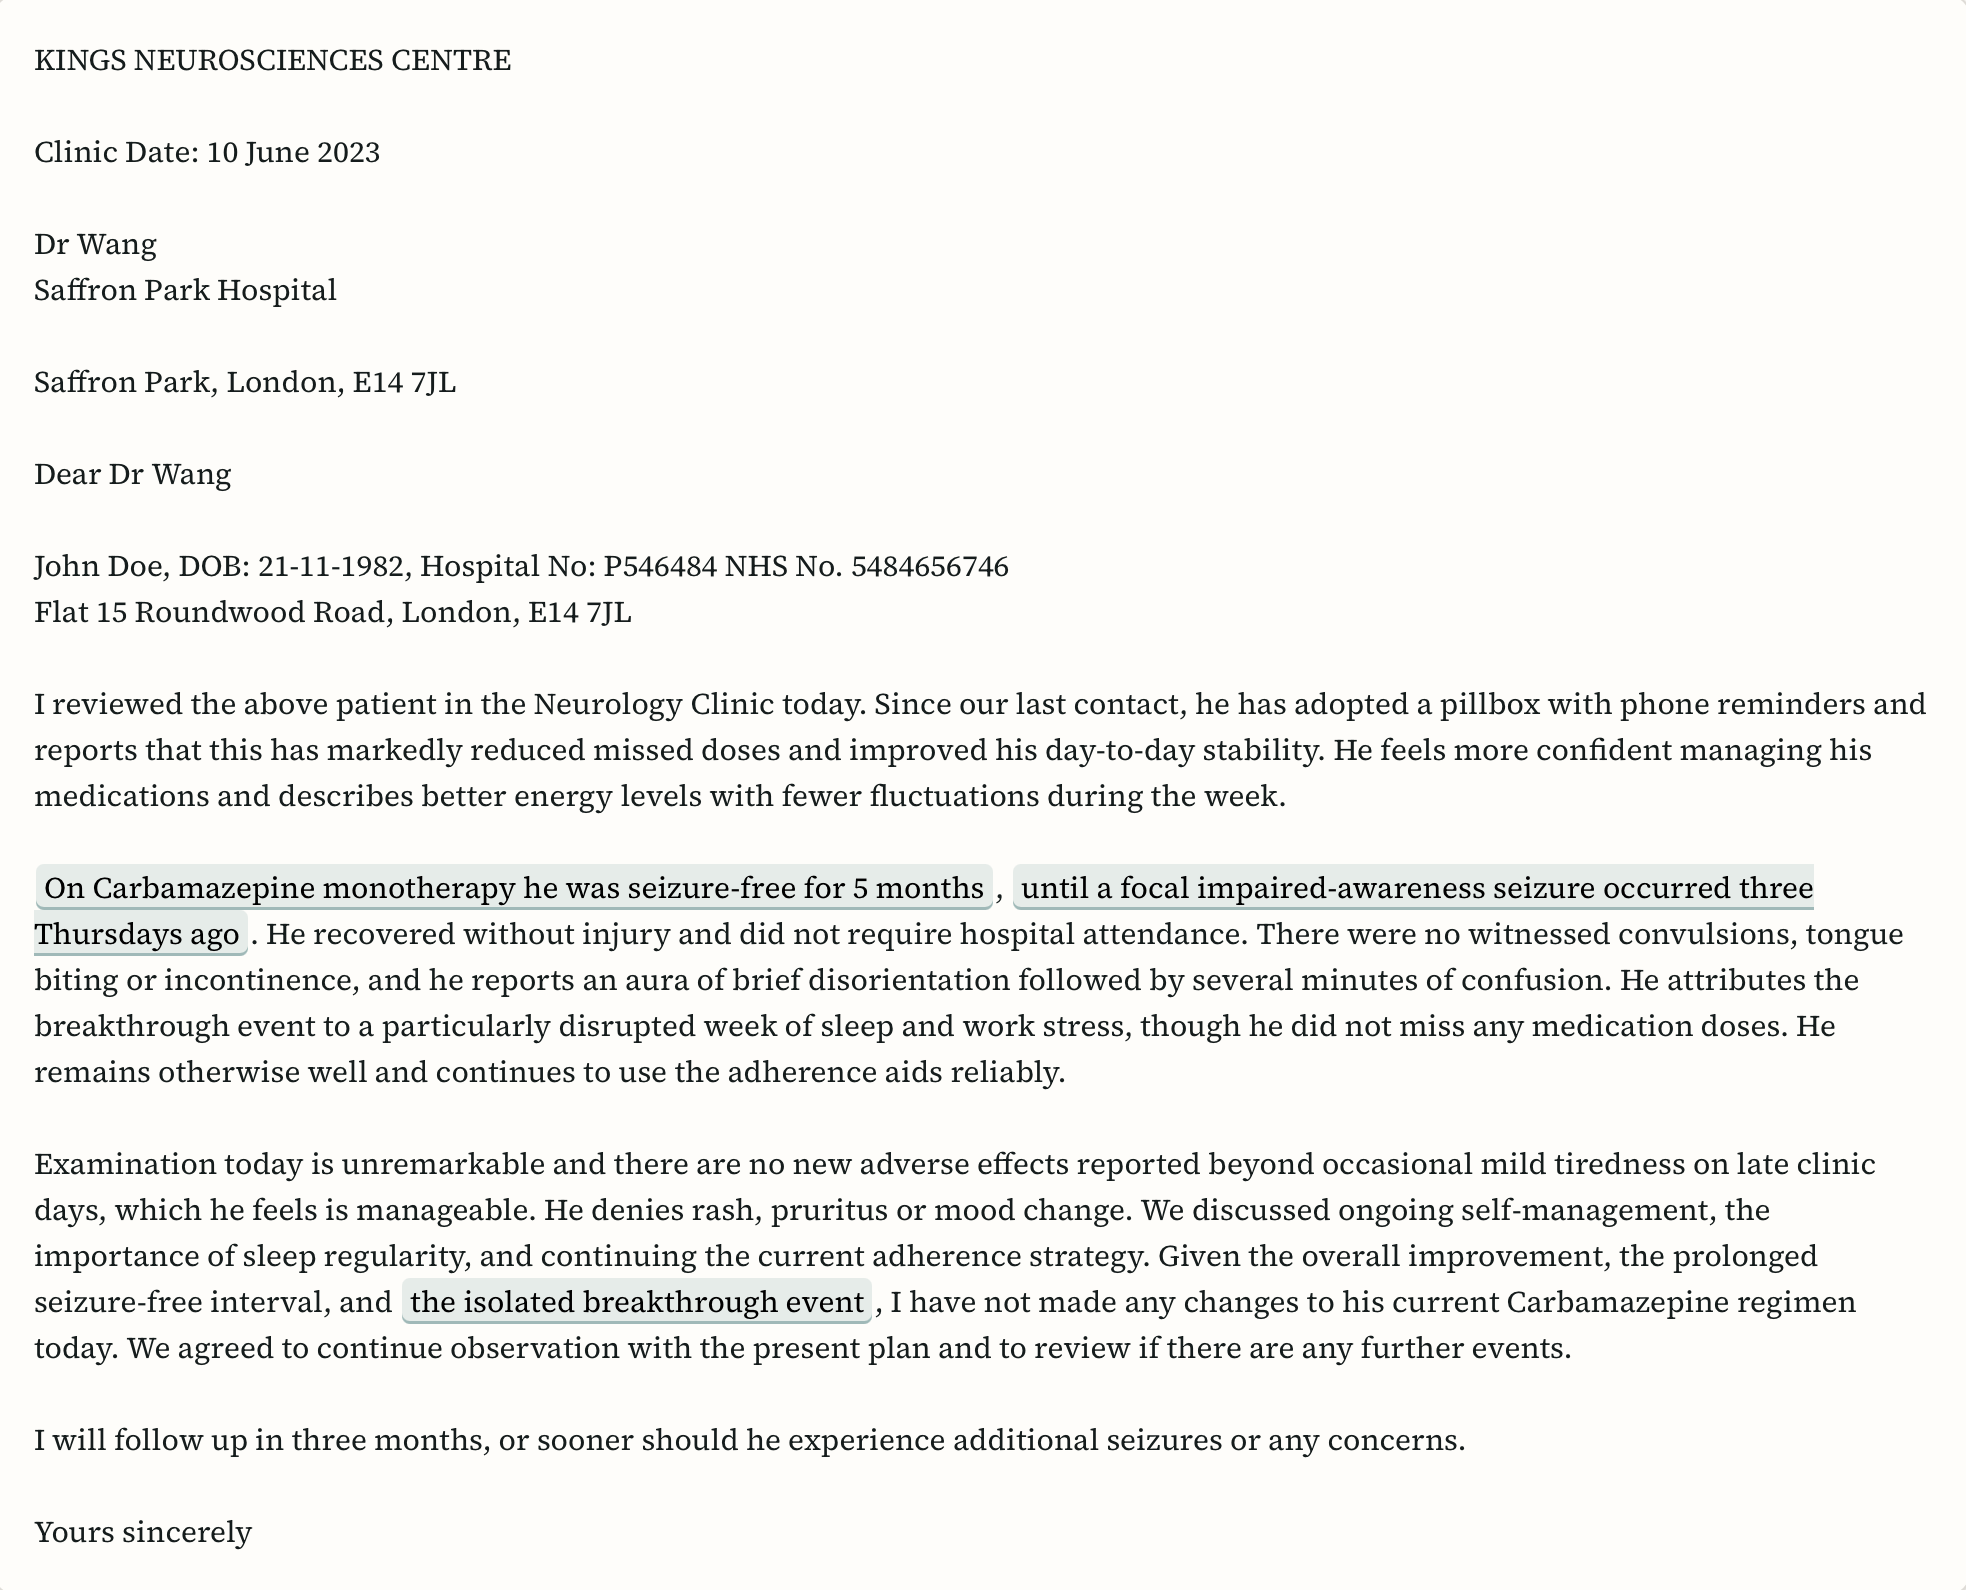
\includegraphics[width=\linewidth]{fig2.png}
    \caption{A clinic letter passes through three stages in the pipeline - recognise, encode and select - to generate structured labels with the exact text used from the letter to produce the label. Each of the three stages can be configured to use an LLM, rules or both. The example shown is the task of extracting a single label representing the patient's current seizure frequency burden.}
    \label{fig2}
\end{figure*}

\begin{table}[!t]
\caption{Pipeline configurations}
\label{tab:pipeline}
\centering
\begin{tabularx}{\linewidth}{|Y|Y|Y|Y|}
\hline
\textbf{Configuration} &
\textbf{Recognise} &
\textbf{Encode} &
\textbf{Select} 
 \\
\hline

Rules only & 
Rules & 
Rules & 
Rules \\
\hline

LLM + Rules & 
LLM & 
LLM + Rules & 
Rules \\
\hline

LLM only & 
LLM & 
LLM & 
LLM \\
\hline

\end{tabularx}
\end{table}

\subsection{Study Design}

The primary objective of this research is to identify which 
component performs best at which stage. Table 2 shows 
the 3 pipeline configurations used in the evaluation: rules
at every stage, the LLM at every stage or a combination
of LLM and rules. For each configuration we evaluated 
the pipeline at each stage: recognise, encode and select.
This will produce a 3x3 matrix of results that answer two
key questions: 

\begin{enumerate}
\item Among the three pipeline configurations, which performs
best: rules, LLM, or a combination of both?
\item How much incremental value is there from the additional
encode and select stages?
\end{enumerate}

Evaluating the pipeline on both datasets provides insight
into whether this method generalises to both single and 
multi-label prediction tasks with distinctly different challenges. 
Past research has shown that individual methods which perform 
well on extracting a broad clinical inventory perform worst on
extracting seizure frequency, and methods that extract seizure
frequency effectively on one corpus generalise poorly to 
another corpus with a different structure and writing style.

For the inventory task, the challenging part is finding the 
right balance between precision and recall. On average there are 
6 labels per letter to extract, but some letters have 0 and some have 14. In this 
scenario it would be easy to tune a pipeline that either 
over-extracts when there  is an absence of real 
evidence(false positives) or under-extracts when there is 
an abundance of evidence (false negatives). The benefit of 
breaking the task into three stages is that you can then tune 
each stage accordingly. The candidate recognition phase can 
be tuned to maximise recall at the cost of some precision, 
recognising a high number of true positives with a reasonable 
number of false positives. The selection phase can then be
tuned for precision to filter out the false positives. We can
then evaluate whether LLMs or rules perform best at each 
task.

For the current frequency dataset, the challenging part is 
determining which one fact among many is the correct 
answer. Sometimes that requires grouping together 
multiple related facts into a single answer, e.g. '1 in
June, 0 in July, 2 in August' becomes '3 in 3 months'. 
Sometimes it requires determining which fact takes 
precedence when there are multiple competing facts with 
varying degrees of specificity and certainty e.g. 'She may 
remain seizure-free for up to 4 month, but then will 
experience clusters of 5 seizures in a single day'. Different 
annotation guidelines would record ambiguous facts like 
these differently. Distinct stages in the pipeline make 
those choices configurable and explicit.

The primary hypothesis is that a combination of an LLM
plus rules will perform better than either on their own, 
because they have complementary strengths and those 
strengths are particularly well suited to distinct stages in
the pipeline. The secondary hypothesis is that multiple 
discrete stages will improve performance for the LLM,
whether the subsequent stages are rules or additional
LLM calls. This builds on the idea that task decomposition
is an effective form of context engineering, and is 
particularly useful in scenarios where the prompt is long
and contains many layers of instructions. 

Splitting the pipeline into stages is therefore designed to 
make it easier to evaluate and easier to optimise, producing 
better results overall.

\subsection{Pipeline Optimisation}

Over 50 evaluations were conducted on the development set 
to optimise the two key elements of the pipeline: the LLM
prompt instructions and the rules. The focus of the optimisation 
process was to optimise accuracy, precision, recall or the F1 
score, depending on the task and stage. In-depth qualitative 
error analysis was conducted to diagnose the cause of poor
performance in particular areas and identify common error 
modes. Hypotheses were developed and tested to tune the 
prompt and rules iteratively. 

Multiple configurations of the overall architecture 
were explored in the early stages, particularly for the 
LLM component. Three distinct architectures were: 

\begin{enumerate}
\item Task specialisation: breaking up the inventory task into 
individual prompts for each clinical family.
\item Document splitting: splitting up the document into discrete
sections and providing targeted instructions for each section.
\item Generator-verifier: using the first LLM to provide the answers 
and an LLM-as-a-judge to verify them.
\end{enumerate}

All configurations were based on the assumption that 
the LLM could provide the best answer in a single prompt,
as this was the common design in the literature. Through
iterative error analysis on both the LLM and the rules,
it became apparent that the complexity of the task was 
more often a function of competing rules and guidelines
on the same clinical family, rather than the breadth of rules
across families. Often improving a rule or a prompt 
instruction to address one class of error would harm 
another area because annotation policies are complex 
and can appear contradictory in some instances. This 
complexity is a challenge for human annotators also, 
as described above in the literature review.

Decomposing the task into three stages allowed for 
cleaner separation of the polices on which types of 
facts to extract and which criteria to apply to exclude
specific variants of them. Decomposing the task into
three stages also made it possible to evaluate the 
performance at each individual and clear identify the 
bottlenecks in the system. It is this combination of 
a cleaner task decomposition for the pipeline and a
clearer view into the pipeline that enabled steady,
incremental gains to materialise from the optimisation
process.

\subsection{Evaluation}

REMOVE DEFENSIVE LANGUAGE AND CAVEATS, SPEAK PLAINLY

The pipeline was evaluated using a single 
headline metric for each dataset: the micro-F1 
score for inventory and accuracy for current frequency. 
The reason the two datasets use two different 
headline metrics is because current frequency only 
contains a single label for each letter, while inventory 
contains an average of 6 labels per letter. Simple
accuracy is sufficient for a single label, but
multi-label predictions require a more sophisticated
metric to evaluate performance.

Accuracy measures how often the correct answer
was selected out of all answers provided. In 
the current frequency task, there is only one
answer per letter so accuracy is a complete 
measurement of how often the pipeline selected
the correct answer. Before computing the 
accuracy, Gan \emph{et. al} categorised the 
monthly frequency rates into two groups: a 
fine-grained category called 'purist' and a coarse
category called 'pragmatic'. For example, the 
label '1 per month' was assigned to the purist 
group 'monthly, not weekly' and the pragmatic
group 'frequent'. This paper uses purist accuracy 
as the primary metric for current frequency 
because distinguishing between daily and 
monthly seizures is a clinically important detail.

The micro-F1 score is used for inventory as it 
measures how well the pipeline can accurately 
extract facts from all four clinical categories.  
The F1 score measures the harmonic mean of
precision and recall. Recall measures how many
of the correct answers can be predicted, while
precision measures how often a prediction is
correct. Micro-F1 takes the average F1 score 
across each of the categories, in this case 
medication, diagnosis, investigations and 
seizure frequency. The macro-F1 score would 
assign more weight to the diagnosis category
because it contains more labels per letter. The 
micro-F1 score ensures each category is given 
equal importance.

All metrics presented in the paper use the held-out
test sets. This measures how well the pipeline
generalises to examples it has not seen before. The 
development sets were used explicitly to optimise the 
rules and prompts through iterative error analysis 
and performance can be inflated by over-fitting to 
specific patterns in those letters. The held-out test
set is used to reduce that risk and evaluate how 
well the pipeline can identify meaningful patterns.
Letters from the development set are used in this 
paper to show how a prediction moves through each 
of the stages in the pipeline and the evidence chain 
it is connected to, or to illustrate a particular type of 
error.

\section{Results}
\subsection{Development Environment}



\subsection{Methods}

For the inventory task the
three-stage lens made it clear that the major limiting factor
was low recall at the recognition phase. Precision was
consistently high but the prompt instructions were causing
too many valid candidates to be excluded in a single 
extraction call. Using more permissive guidelines in
the recognition phase significantly improved recall at
the cost of some precision, but the select phase was 
able to recover that precision. 

\subsection{Models}
\subsection{Structured Evidence}
\subsection{Ablations}
\subsection{Error Analysis}

\section{Discussion}

\section{Conclusion}


\section*{References}

Please number citations consecutively within brackets \cite{b1}. The 
sentence punctuation follows the bracket \cite{b2}. 

\begin{thebibliography}{00}
\bibitem{b1} B. Fonferko-Shadrach \emph{et al.}, ``Using natural language processing to extract structured epilepsy data from unstructured clinic letters: development and validation of the ExECT (extraction of epilepsy clinical text) system,'' \emph{BMJ Open}, vol.~9, no.~4, 2019, Art.~no.~e023232.
\bibitem{b2} B. Fonferko-Shadrach \emph{et al.}, ``Annotation of epilepsy clinic letters for natural language processing,'' \emph{J. Biomed. Semantics}, vol.~15, no.~17, 2024.
\bibitem{b3} Y. Gan \emph{et al.}, ``Reproducible synthetic clinical letters for seizure frequency information extraction,'' arXiv:2603.11407, 2026.
\bibitem{b4} K. Xie \emph{et al.}, ``Extracting seizure frequency from epilepsy clinic notes: a machine reading approach to natural language processing,'' \emph{J. Amer. Med. Informat. Assoc.}, vol.~29, no.~5, pp.~873--881, 2022.
\bibitem{b5} B. Holgate, J. Davies, S. Fang, J.~S. Winston, J.~T. Teo, and M.~P. Richardson, ``Fine-tuning LLMs to extract epilepsy seizure frequency data from health records,'' in \emph{Proc. 24th Workshop on Biomedical Language Processing (BioNLP)}, 2025, pp.~44--55.
\bibitem{b6} S. Fu \emph{et al.}, ``Clinical concept extraction: A methodology review,'' \emph{J. Biomed. Informat.}, vol.~109, 2020, Art.~no.~103526.
\bibitem{b7} R. Grishman and B. Sundheim, ``Message Understanding Conference-6: A brief history,'' in \emph{Proc. 16th Int. Conf. Computational Linguistics (COLING)}, 1996, pp.~466--471.
\bibitem{b8} Y. Wang \emph{et al.}, ``Clinical information extraction applications: A literature review,'' \emph{J. Biomed. Informat.}, vol.~77, pp.~34--49, 2018.
\bibitem{b9} K. Xie, B. Litt, D. Roth, and C.~A. Ellis, ``Quantifying clinical outcome measures in patients with epilepsy using the electronic health record,'' in \emph{Proc. BioNLP Workshop}, 2022, pp.~369--375.
\bibitem{b10} M. Agrawal, S. Hegselmann, H. Lang, Y. Kim, and D. Sontag, ``Large language models are few-shot clinical information extractors,'' in \emph{Proc. Conf. Empirical Methods in Natural Language Processing (EMNLP)}, 2022, pp.~1998--2022.
\bibitem{b11} L. Chiticariu, Y. Li, and F. Reiss, ``Rule-based information extraction is dead! Long live rule-based information extraction systems!,'' in \emph{Proc. Conf. Empirical Methods in Natural Language Processing (EMNLP)}, 2013, pp.~827--832.
\bibitem{b12} B.~M. Decker \emph{et al.}, ``Development of a natural language processing algorithm to extract seizure types and frequencies from the electronic health record,'' \emph{Seizure}, vol.~101, pp.~48--51, 2022.
\bibitem{b13} interoperability-standard-contract
\end{thebibliography}

\vspace{12pt}

\end{document}
